\PassOptionsToPackage{table}{xcolor}
\documentclass[10pt]{beamer}

\usetheme[progressbar=frametitle]{metropolis}
\usepackage{appendixnumberbeamer}

\usepackage{booktabs}
\usepackage[scale=2]{ccicons}

\usepackage{pgfplots}
\usepgfplotslibrary{dateplot}

\usepackage{xspace}
\newcommand{\themename}{\textbf{\textsc{metropolis}}\xspace}

\usepackage[brazilian]{babel}
\usepackage[utf8]{inputenc}
\usepackage[T1]{fontenc}
\usepackage{multirow}

\usepackage[table]{xcolor}
\usepackage{pgfplots}
\usepackage{pifont}

\newcommand*\rot{\rotatebox{90}}
\newcommand*\V{\ding{51}}

\title{UNIVERSIDADE DE ITAÚNA}
\subtitle{Aprendizado de Máquina Aplicado à Valoração de Redações}
% \date{\today}
\date{19 de Junho de 2017}
\author{\textbf{Graduando:} Eugênio Cunha \\ \textbf{Orientador:} Dr. Marco Túlio Alves N Rodrigues}
\institute{{Departamento de Ciência da Computação \small} \\ {Bacharelado em Ciência da Computação \small}}
\titlegraphic{\hfill
\includegraphics[height=1.5cm]{images/uit.pdf}}

\begin{document}

\maketitle

\begin{frame}{Aprendizado de Máquina Aplicado à Valoração de Redações}
  \setbeamertemplate{section in toc}[sections numbered]
  \tableofcontents[subsectionstyle=show]
\end{frame}

\section{Introdução}

  \subsection{Problema de Pesquisa}
    \begin{frame}[fragile]{Problema de Pesquisa}
    O decreto 79.298, de 24 de Fevereiro de 1977 definiu a “inclusão obrigatória da prova ou questão de redação em língua portuguesa” nos concursos e vestibulares (Art. 1 o , alínea d).
    \end{frame}

    \begin{frame}[fragile]{Problema de Pesquisa}
    No ENEM cada redação é avaliada por, pelo menos, dois avaliadores, de forma independente ~\cite{edital_enem:2016}.
    \begin{figure}[H]
    \begin{center}
        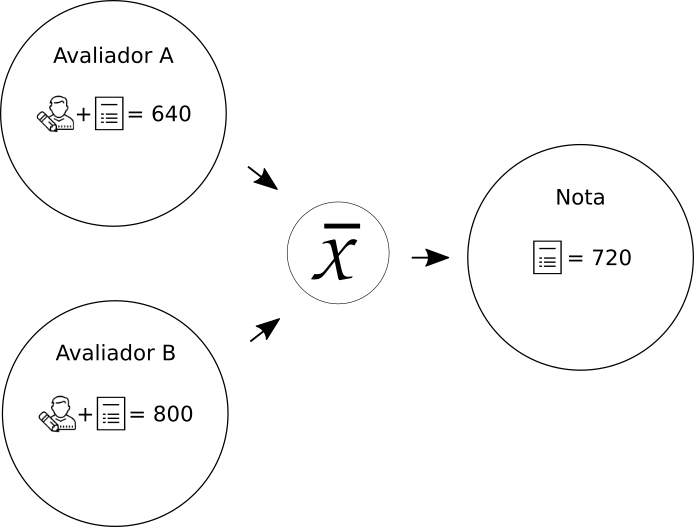
\includegraphics[scale=0.50]{images/correction_redaction_enem.png}
    \end{center}
    \end{figure}
    \end{frame}

    \begin{frame}[fragile]{Problema de Pesquisa}
    Dados da avaliação de redações do ENEM 2016 ~\cite{paq_a:2016}.
    \begin{figure}[H]
    \begin{center}
        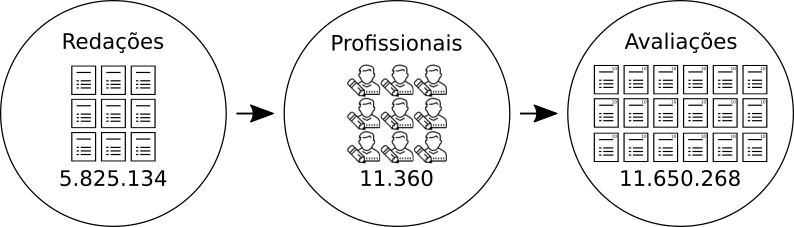
\includegraphics[scale=0.50]{images/enem_2016.png}
    \end{center}
    \end{figure}
    \end{frame}

    \begin{frame}[fragile]{Problema de Pesquisa}
    Dado um corpus de redações, classificar as competências exigidas em um texto de redação.
    \begin{figure}[H]
    \begin{center}
        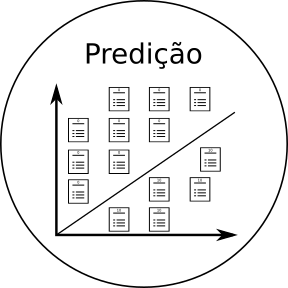
\includegraphics[scale=0.50]{images/prediction.png}
    \end{center}
    \end{figure}
    \end{frame}

  \subsection{Objetivos}
    \begin{frame}[fragile]{Objetivos}
    Induzir um modelo de Aprendizado de Máquina a classificar as competências exigidas em um texto de redação.

    \begin{figure}[H]
    \begin{center}
        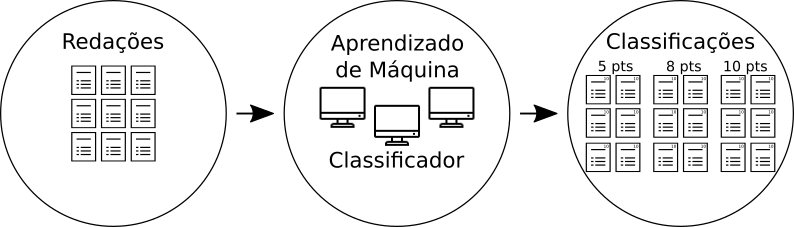
\includegraphics[scale=0.50]{images/automatic_essay_system.png}
    \end{center}
    \end{figure}
    \end{frame}

  \subsection{Motivação}
    \begin{frame}[fragile]{Motivação}
    Aprendizado de Máquina está no centro de muitos avanços tecnológicos, alcançado áreas antes exclusivas de seres humanos.
    \begin{figure}[H]
    \begin{center}
        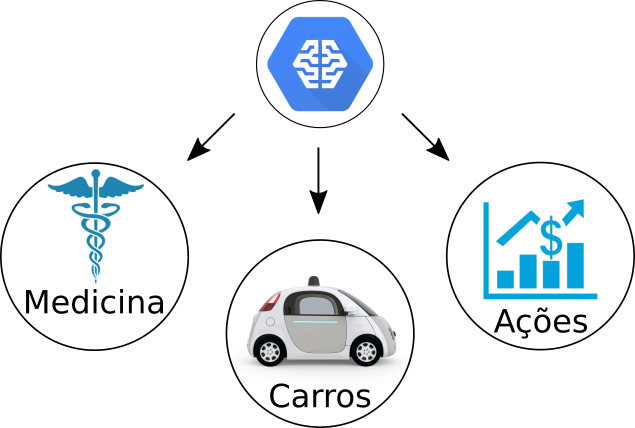
\includegraphics[scale=0.50]{images/machine_learn.png}
    \end{center}
    \end{figure}
    \end{frame}

\section{Trabalhos Relacionados}
  \begin{frame}[fragile]{Matriz de Competências}
  Silva (2017) cita em seu estudo, que à prova de redação do ENEM é avaliada levando em conta uma matriz de referência elaborada pelo INEP ~\cite{silvio_taynan:2017}.
  \begin{table}[H]
  \centering
  \begin{tabular}{|c|l|c|}
  \hline
  \textbf{I} & {Demonstrar domínio da norma padrão da língua escrita.}\small & 200 \\ \hline
  \textbf{II} & \begin{tabular}[c]{@{}l@{}}Compreender a proposta de redação e aplicar conceitosdas \\ varias áreas de conhecimento para desenvolver o tema, dentro \\ dos limites estruturais do textodissertativo-argumentativo em \\ prosa.\end{tabular} & 200 \\ \hline
  \textbf{III} & \begin{tabular}[c]{@{}l@{}}Selecionar, relacionar, organizar e interpretar informações, \\ fatos, opiniões e argumentos em defesa de um ponto de vista.\end{tabular} & 200 \\ \hline
  \textbf{IV} & \begin{tabular}[c]{@{}l@{}}Demonstrar conhecimento dos mecanismos linguísticos \\ necessários para a construção da argumentação.\end{tabular} & 200 \\ \hline
  \textbf{V} & \begin{tabular}[c]{@{}l@{}}Elaborar proposta de intervenção para o problema abordado, \\ respeitando os direitos humanos.\end{tabular} & 200 \\ \hline
  \end{tabular}
  \end{table}
  \end{frame}

  \begin{frame}[fragile]{Aprendizado de Máquina}
    Segundo Monard (2003), de uma forma geral o aprendizado indutivo pode ser dividido em supervisionado e não-supervisionado ~\cite{monard_baranauskas:2003}.
    \begin{figure}[H]
    \begin{center}
        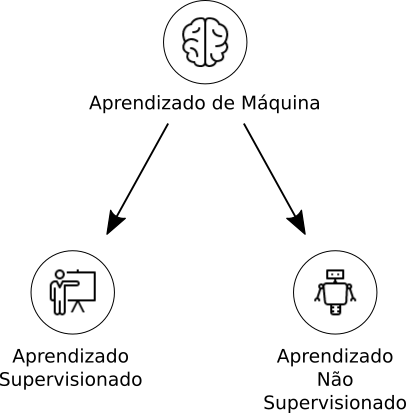
\includegraphics[scale=0.45]{images/supervised_unsupervised.png}
    \end{center}
    \end{figure}
    Freitas (2005), cita que o aprendizado supervisionado exige como entrada um corpus de treino, com exemplos corretamente rotulados ~\cite{de2005anotaccao}.
  \end{frame}

  \begin{frame}[fragile]{Aprendizado de Máquina}
    \begin{center}
    \textbf{Supervisionado ou não-supervisionado?}
    \end{center}
    \begin{table}[]
    \centering
    \begin{tabular}{|r|l|}
    \hline
    \textbf{Tema} & \textit{Direitos em conflito: liberdade de expressão e ...} \\ \hline
    \textbf{Título} & \textit{Os limites da informação} \\ \hline
    \textbf{Texto} & \textit{Analisando todo um conjunto de fatos importantes ...} \\ \hline
    \textbf{Competência I} & 50 \\ \hline
    \textbf{Competência II} & 100 \\ \hline
    \textbf{Competência III} & 50 \\ \hline
    \textbf{Competência IV} & 50 \\ \hline
    \textbf{Competência V} & 50 \\ \hline
    \textbf{Nota Total} & \textbf{300} \\ \hline
    \end{tabular}
    \caption{Propriedades de uma redação.}
    \end{table}
    \begin{center}
      \textbf{Aprendizado supervisionado.}
    \end{center}
  \end{frame}

  \begin{frame}[fragile]{Aprendizado de Máquina}
    De acordo com o estudo de Monard (2003) o aprendizado supervisionado pode ser induzido a resolver problemas de classificação ou regressão ~\cite{monard_baranauskas:2003}.
    \begin{figure}[H]
    \begin{center}
        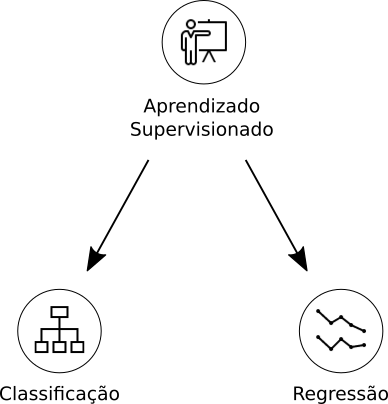
\includegraphics[scale=0.45]{regression_classification.png}
    \end{center}
    \end{figure}
    O autor ainda cita, ``Para rótulos de classe discretas, esse problema é conhecido como classificação e para valores contínuos como regressão.''
  \end{frame}

  \begin{frame}[fragile]{Aprendizado de Máquina}
    \begin{center}
    \textbf{Classificação ou Regressão?}
    \end{center}

    \begin{table}[H]
    \centering
    \begin{tabular}{|l|l|c|c|c|}
    \hline
    \multicolumn{2}{|c|}{\textbf{Competência}} & \multicolumn{1}{l|}{\textbf{Valor}} & \multicolumn{1}{l|}{\textbf{Subitens}} & \multicolumn{1}{l|}{\textbf{Valor/Classes}} \\ \hline
    \multirow{2}{*}{} & \multirow{2}{*}{} & \multirow{2}{*}{} & \textit{0} & \textbf{0} \\ \cline{4-5} 
     &  &  & \textit{1} & \textbf{50} \\ \hline
    \textbf{I} & \textit{\begin{tabular}[c]{@{}l@{}}Demonstrar domínio da norma\\  padrão da língua escrita.\end{tabular}} & \textbf{200} & \textit{2} & \textbf{100} \\ \hline
    \multirow{2}{*}{} & \multirow{2}{*}{} & \multirow{2}{*}{} & \textit{3} & \textbf{150} \\ \cline{4-5} 
     &  &  & \textit{4} & \textbf{200} \\ \hline
    \end{tabular}
    \caption{Competência I da matriz de referência.}
    \end{table}
    \begin{center}
      \textbf{Problema de classificação.}
    \end{center}
  \end{frame}

  \begin{frame}[fragile]{\textit{Boost} -> \textit{AdaBoost}}
    O AdaBoost é um algoritmo de aprendizado supervisionado do tipo \textit{Boost}, que combina um conjunto de funções simples de classificação, denominadas classificadores fracos para formar um classificador forte.

    \begin{figure}[H]
    \begin{center}
        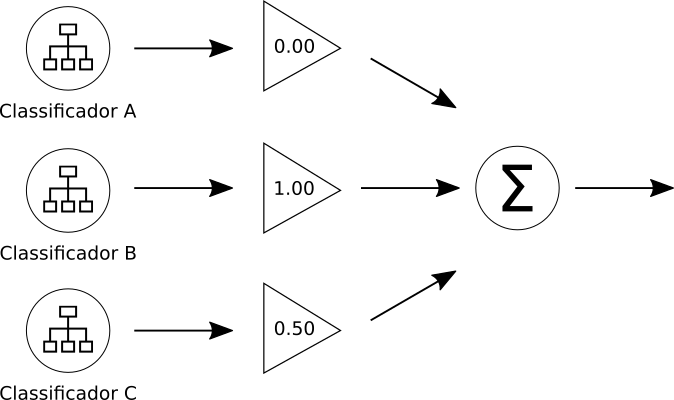
\includegraphics[scale=0.35]{images/boosting.png}
    \end{center}
    \end{figure}

    Em cada iteração, o procedimento de atualização aumenta os pesos das amostras classificadas incorretamente, fornecendo desta forma a característica adaptativa do AdaBoost.

  \end{frame}

  \begin{frame}[fragile]{Ferramentas}
    Wahbeh et al. (2011) realizou um estudo comparativo entre quatro ferramentas para mineração de dados: KMINE, Orange, Tanagra e Weka ~\cite{wahbeh2011comparison}.

    \begin{figure}[H]
    \begin{center}
        
\includegraphics[scale=0.45]{images/tools_data_mining.png}
    \end{center}
    \end{figure}

    Segundo seu trabalho, ferramenta Weka apresentou o melhor desempenho, seguido pela \textit{Orange}.
  \end{frame}

  \begin{frame}[fragile]{\textit{Orange Data Mining}}
    \begin{figure}[H]
    \begin{center}
        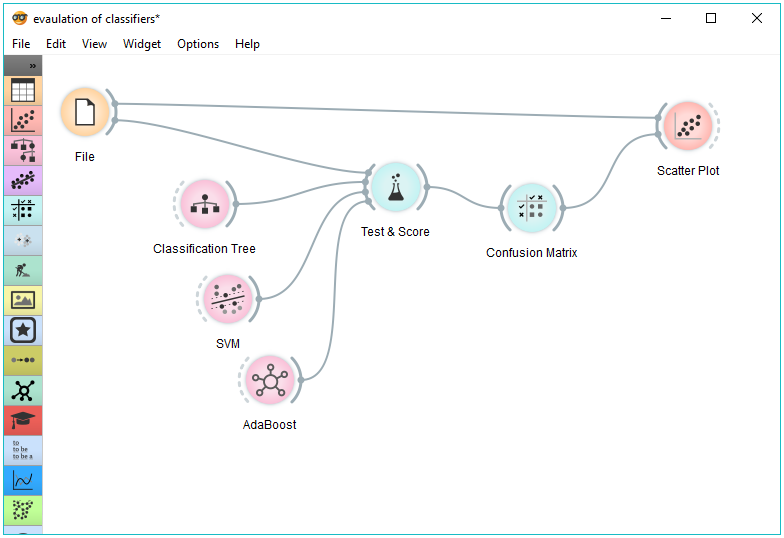
\includegraphics[scale=0.35]{images/orange_canvas.png}
    \end{center}
    \caption{\textit{Orange Data Mining}}
    \end{figure}
  \end{frame}



\section{Metodologia}
  \begin{frame}[fragile]{Coleta de Dados}
  Coletar textos de redações avaliadas segundo a matriz de referência do INEP, normalizar os textos sem alterar o seu valor textual e armazená-lo de forma estruturada, separando o tema, título, texto e nota.
  \begin{figure}[H]
  \begin{center}
      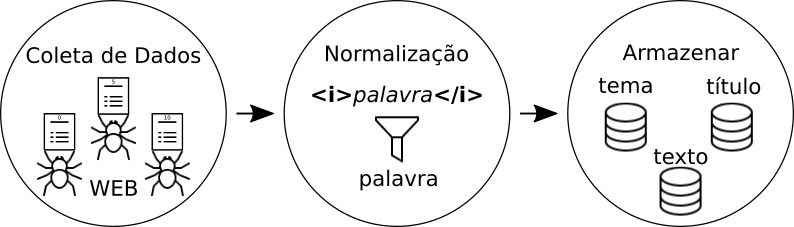
\includegraphics[scale=0.50]{images/methodology_1.png}
  \end{center}
  \end{figure}

  \end{frame}

  \begin{frame}[fragile]{Orange Data Mining}
   Desenvolver uma representação do domínio do problema com auxílio da ferramenta \textit{Orange Data Mining}, induzir o classificado\textit{AdaBoost} sobre a base de conhecimento rotulada, avaliar as métricas de desempenho e repetir o ciclo se necessário.
  \begin{figure}[H]
  \begin{center}
      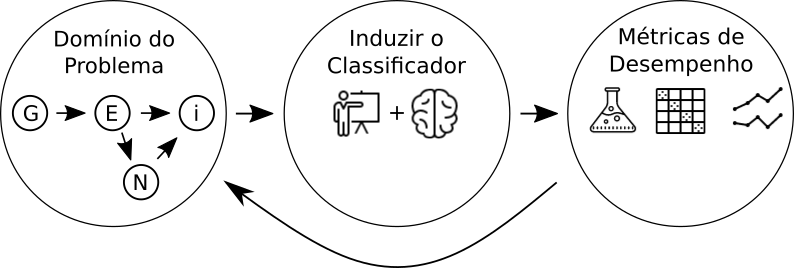
\includegraphics[scale=0.50]{images/methodology_2.png}
  \end{center}
  \end{figure}
  \end{frame}

\section{Resultados Preliminares}
  \begin{frame}[fragile]{Adversidades}
    % A qualidade dos dados no \textit{dataset} é uma fator fundamental.
    Trabalhar com dados desbalanceados tende à produzir regras de classificação que beneficiam as classes majoritárias, resultando em uma baixa taxa de predição para o grupo minoritário.

    \pgfplotstableread[row sep=\\,col sep=&]{
        class & score  \\
        0.00  & 15 \\
        0.50  & 40 \\
        1.00  & 52 \\
        1.50  & 20 \\
        2.00  & 4  \\
        }\mydata

    \begin{figure}[H]
    \begin{center}
    \begin{tikzpicture}
        \begin{axis}[
                ybar,
                width=8cm,
                height=6cm,
                symbolic x coords={0.00,0.50,1.00,1.50,2.00},
                bar width=10pt,
                ylabel=Quantidade,
                % xlabel=Classes,
                xtick=data,
                axis lines*=left,
            ]
            \addplot[draw=black, fill=white] table[x=class,y=score]{\mydata};
            \node [above] at (axis cs:  0.00,15) {15};
            \node [above] at (axis cs:  0.50,40) {40};
            \node [above] at (axis cs:  1.00,52) {52};
            \node [above] at (axis cs:  1.50,20) {20};
            \node [above] at (axis cs:  2.00,4) {4};
        \end{axis}
    \end{tikzpicture}
    \end{center}
    \end{figure}
    \begin{center}
    \textbf{Gráfico 1}: Amostra de 30\% dos dados no \textit{dataset}.
    \end{center}
  \end{frame}

  \begin{frame}[fragile]{Métricas de Desempenho}
    A Tabela ~\ref{tab:evaluation_result} exibe os resultados das principais métricas de desempenho para classificadores e a média geral de cada métrica.

    \begin{table}[H]
    \centering
    \begin{tabular}{c|c|c|c|c|c|}
    \cline{2-6}
     & \multicolumn{5}{c|}{\textbf{Resultado da avaliação}} \\ \hline
    \multicolumn{1}{|c|}{\textbf{Classes}} & \textbf{ROC} & \textbf{Acurácia} & \textit{\textbf{F-Score}} & \textit{\textbf{Precision}} & \textit{\textbf{Recall}} \\ \hline
    \multicolumn{1}{|c|}{\textbf{0.00}}  & 0.498 & 0.828 & 0.096 & 0.845 & 0.828 \\ \hline
    \multicolumn{1}{|c|}{\textbf{0.50}}  & 0.552 & 0.640 & 0.349 & 0.653 & 0.640 \\ \hline
    \multicolumn{1}{|c|}{\textbf{1.00}}  & 0.499 & 0.509 & 0.422 & 0.506 & 0.509 \\ \hline
    \multicolumn{1}{|c|}{\textbf{1.50}}  & 0.549 & 0.579 & 0.222 & 0.755 & 0.759 \\ \hline
    \multicolumn{1}{|c|}{\textbf{2.00}}  & 0.541 & 0.915 & 0.140 & 0.899 & 0.915 \\ \hline
    \multicolumn{1}{|c|}{\textbf{Média}} & \textbf{0.529} & \textbf{0.694} & \textbf{0.246} & \textbf{0.737} & \textbf{0.730} \\ \hline
    \end{tabular}
    \caption{Resultado das métricas de desempenho do classificador AdaBoost.}
    \label{tab:evaluation_result}
    \end{table}
  \end{frame}

  \begin{frame}[fragile]{Matriz de Confusão}
    A Tabela ~\ref{tab:matrix_confusion} exibe ao longo da diagonal em tons de cinza as decisões corretas: número de verdadeiros positivos TP e verdadeiros negativos TN;

    \begin{table}[H]
    \centering
    \begin{tabular}{cc|c|c|c|c|c|c|}
    \cline{3-8}
     &  & \multicolumn{6}{c|}{\textbf{Predição}} \\ \cline{3-8} 
     &  & \textbf{0.00} & \textbf{0.50} & \textbf{1.00} & \textbf{1.50} & \textbf{2.00} & $\sum_{}$  \\ \hline
    \multicolumn{1}{|c|}{} & \textbf{0.00} & \cellcolor[HTML]{C0C0C0}4 & 18 & 13 & 2 & 0 & \textbf{37} \\ \cline{2-8} 
    \multicolumn{1}{|c|}{} & \textbf{0.50} & 13 & \cellcolor[HTML]{C0C0C0}42 & 44 & 14 & 1 & \textbf{114} \\ \cline{2-8} 
    \multicolumn{1}{|c|}{} & \textbf{1.00} & 18 & 51 & \cellcolor[HTML]{C0C0C0}78 & 32 & 11 & \textbf{190} \\ \cline{2-8} 
    \multicolumn{1}{|c|}{} & \textbf{1.50} & 7 & 14 & 31 & \cellcolor[HTML]{C0C0C0}15 & 2 & \textbf{69} \\ \cline{2-8} 
    \multicolumn{1}{|c|}{} & \textbf{2.00} & 4 & 2 & 14 & 3 & \cellcolor[HTML]{C0C0C0}3 & \textbf{26} \\ \cline{2-8} 
    \multicolumn{1}{|c|}{\multirow{-6}{*}{\rot{Atual}}} & $\sum_{}$ & \textbf{46} & \textbf{127} & \textbf{180} & \textbf{66} & \textbf{17} & \textbf{436} \\ \hline
    \end{tabular}
    \caption{Matriz de confusão resultante da indução do classificador \textit{AdaBoost}.}
    \label{tab:matrix_confusion}
    \end{table}
  
  \end{frame}

\section{Plano de Trabalho}
  \begin{frame}[fragile]{Plano de Atividades}
    \begin{center}
    \scalebox{0.9}{
    \rowcolors{1}{}{gray!25}
    \begin{tabular}{c|l|c|c|c|c|c|c|c|c|c|c|}& Atividade & \rot{Fevereiro - 2017} & \rot{Março - 2017} & \rot{Abril - 2017} & \rot{Maio - 2017} & \rot{Junho - 2017} & \rot{Julho - 2017} & \rot{Agosto - 2017} & \rot{Setembro - 2017} & \rot{Outubro - 2017} & \rot{Novembro - 2017} \\
        \hline
        1 & Revisão Bibliográfica    &\V &\V &\V &   &   &   &   &   &   &   \\
        2 & Coleta de Dados          &   &   &   &\V &   &   &   &   &   &   \\
        3 & Tratamento dos Dados     &   &   &   &\V &   &   &   &   &   &   \\
        4 & Domínio do Problema      &   &   &   &   &\V &\V &\V &\V &   &   \\
        5 & Indução do Classificador &   &   &   &   &\V &\V &\V &\V &   &   \\
        6 & Métricas de Desempenho   &   &   &   &   &\V &\V &\V &\V &\V &   \\
        7 & Escrita da Monografia    &\V &\V &\V &\V &\V &\V &\V &\V &\V &\V \\
        8 & Entrega da Monografia    &   &   &   &   &   &   &   &   &   &\V \\
        \hline
    \end{tabular}}
    \end{center}
  \end{frame}

% \appendix desliga o slide da barra de progresso
\appendix
\begin{frame}[allowframebreaks]{References}

  \bibliography{bib}
  \bibliographystyle{abbrv}
\end{frame}

\end{document}